\documentclass[tikz, crop, border=5pt]{standalone}
\usetikzlibrary{positioning,backgrounds,fit,shapes.geometric,calc}

\usepackage{fontspec}
\usepackage{xeCJK}

\setmainfont{NotoSans}[
    Extension      = .ttf,
    UprightFont    = *-Regular,
    BoldFont       = *-Bold,
    ItalicFont     = *-Italic,
    BoldItalicFont = *-BoldItalic
]

\usepackage{color}
\definecolor{black}{RGB}{26,25,25}
\definecolor{grey}{RGB}{129,130,132}
\definecolor{red}{RGB}{188,36,46}
\definecolor{brown}{RGB}{121,37,0}
\definecolor{green}{RGB}{32,128,108}
\definecolor{purple}{RGB}{160,90,150}
\definecolor{blue}{RGB}{0,103,149} % MidnightBlue

\tikzset{
    base/.style={
%COLOR_BEGIN%
        draw=grey,
        fill=grey,
        text=white,
%COLOR_END%
    },
    % Adenylation
    A/.style={
        base,
        circle,
        minimum size=1cm,
        inner sep=0pt,
        anchor=south,
        yshift=-2mm,
    },
    % Condensation
    C/.style={
        base,
        regular polygon,
        regular polygon sides=3,
        shape border rotate=180,
        minimum width=0.9cm,
        inner sep=0pt,
        anchor=north,
        yshift=1mm,
    },
    % Epimerization
    E/.style={
        base,
        regular polygon,
        regular polygon sides=3,
        shape border rotate=0,
        minimum width=0.9cm,
        anchor=south,
        yshift=-1mm,
    },
    % Condensation/Epimerization
    CE/.style={
        base,
        diamond,
        minimum width=0.8cm,
        minimum height=1.19cm,
    },
    % Thiolation
    T/.style={
        base,
        rectangle,
        minimum height=0.5cm,
        minimum width=0.2cm,
        anchor=north,
        yshift=1mm,
    },
    % Thioesterase
    Te/.style={
        base,
        circle,
        minimum width=0.6cm,
        anchor=north,
        yshift=2mm,
    },
    % Reductase
    R/.style={
        base,
        regular polygon,
        regular polygon sides=4,
        minimum width=0.8cm,
        anchor=north,
        yshift=2mm,
    },
    % Methyltransferase
    M/.style={
        base,
        ellipse,
        minimum width=0.9cm,
        minimum height=0.6cm,
    },
}

\begin{document}
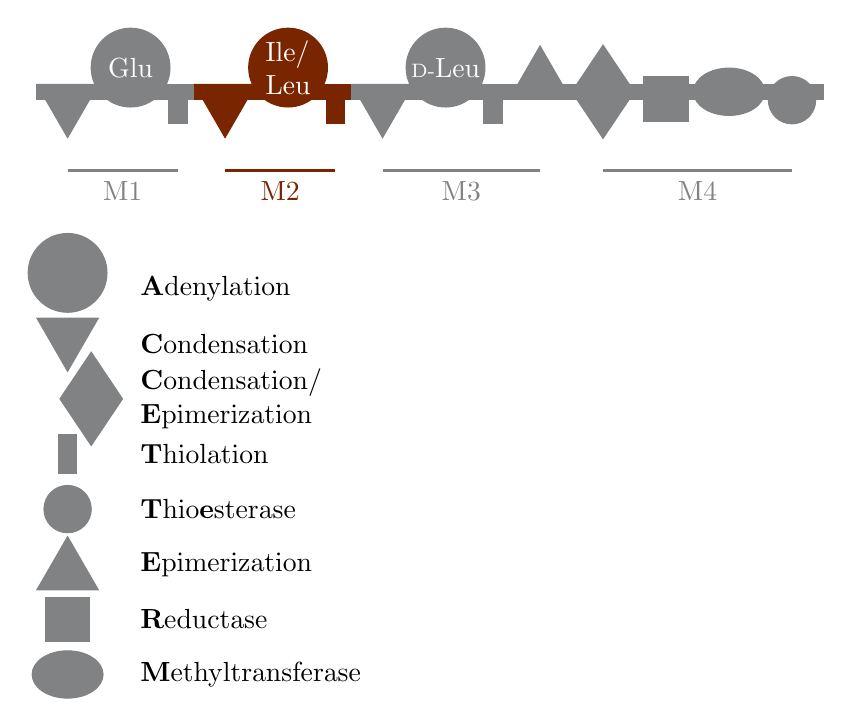
\begin{tikzpicture}
% Define origin point
\coordinate (origin) at (-0.4cm,0);
%MODULE_BEGIN%
    % Draw module sequence
    % M1
    \begin{scope}[shift={([shift={(0.4cm,0)}]origin.east)}] % the leading space for C
        \node[C] (M1-1) at (0,0) {};
        \node[A] (M1-2) at (0.8,0) {};
        \node[text=white,align=left] at (M1-2) {Glu};
        \node[T] (M1-3) at (1.4,0) {};
        \begin{scope}[on background layer]
            \draw[grey, line width=0.5mm, yshift=-1cm]
                let \p1 = (M1-1), \p2 = (M1-3) in
                (\x1,0) -- (\x2,0)
                node[midway, below, text=grey] {M1};
            \draw[grey, line width=2mm]
                let \p1 = (M1-3) in
                (-0.4,0) -- (\x1 + 0.2cm, 0)
                coordinate (M1);
        \end{scope}
    \end{scope}
    % M2
    \begin{scope}[shift={([shift={(0.4cm,0)}]M1.east)}]
        \node[C, brown] (M2-1) at (0,0) {};
        \node[A, brown] (M2-2) at (0.8,0) {};
        \node[text=white,align=left] at (M2-2) {Ile/\\Leu};
        \node[T, brown] (M2-3) at (1.4,0) {};
        \begin{scope}[on background layer]
            \draw[brown, line width=0.5mm, yshift=-1cm]
                let \p1 = (M2-1), \p2 = (M2-3) in
                (\x1,0) -- (\x2,0)
                node[midway, below, text=brown] {M2};
            \draw[brown, line width=2mm]
                let \p1 = (M2-3) in
                (-0.4,0) -- (\x1 + 0.2cm,0)
                coordinate (M2);
        \end{scope}
    \end{scope}
    % M3
    \begin{scope}[shift={([shift={(0.4cm,0)}]M2.east)}]
        \node[C] (M3-1) at (0,0) {};
        \node[A] (M3-2) at (0.8,0) {};
        \node[text=white] at (M3-2) {{\scriptsize D-}Leu};
        \node[T] (M3-3) at (1.4,0) {};
        \node[E] (M3-4) at (2,0) {};
        \begin{scope}[on background layer]
            \draw[grey, line width=0.5mm, yshift=-1cm]
                let \p1 = (M3-1), \p2 = (M3-4) in
                (\x1,0) -- (\x2,0)
                node[midway, below, text=grey] {M3};
            \draw[grey, line width=2mm]
                let \p1 = (M3-4) in
                (-0.4,0) -- (\x1 + 0.4cm, 0)
                coordinate (M3);
        \end{scope}
    \end{scope}
    % M4
    \begin{scope}[shift={([shift={(0.4cm,0)}]M3.east)}]
        \node[CE] (M4-1) at (0,0) {};
        \node[R] (M4-2) at (0.8,0) {};
        \node[M] (M4-3) at (1.6,0) {};
        \node[Te] (M4-4) at (2.4,0) {};
        \begin{scope}[on background layer]
            \draw[grey, line width=0.5mm, yshift=-1cm]
                let \p1 = (M4-1), \p2 = (M4-4) in
                (\x1,0) -- (\x2,0)
                node[midway, below, text=grey] {M4};
            \draw[grey, line width=2mm]
                let \p1 = (M4-4) in
                (-0.4,0) -- (\x1 + 0.4cm, 0)
                coordinate (M4);
        \end{scope}
    \end{scope}
%MODULE_END%

%LEGEND_BEGIN%
    \begin{scope}[yshift=-2.5cm]
        \begin{scope}[yshift=0cm]
            \node[A,anchor=center,yshift=4mm,] at (0,0) {};
            \node[anchor=west] at (0.8,0) {\textbf{A}denylation};
        \end{scope}

        \begin{scope}[yshift=-0.7cm]
            \node[C,anchor=center] at (0,0) {};
            \node[anchor=west] at (0.8,0) {\textbf{C}ondensation};
        \end{scope}

        \begin{scope}[yshift=-1.4cm]
            \node[CE] at (0.3,0) {};
            \node[anchor=west,align=left] at (0.8,0) {\textbf{C}ondensation/\\\textbf{E}pimerization};
        \end{scope}

        \begin{scope}[yshift=-2.1cm]
            \node[T,anchor=center,yshift=-1mm,] at (0,0) {};
            \node[anchor=west] at (0.8,0) {\textbf{T}hiolation};
        \end{scope}

        \begin{scope}[yshift=-2.8cm]
            \node[Te,anchor=center,yshift=-2mm,] at (0,0) {};
            \node[anchor=west] at (0.8,0) {\textbf{T}hio\textbf{e}sterase};
        \end{scope}

        \begin{scope}[yshift=-3.5cm]
            \node[E,anchor=center] at (0,0) {};
            \node[anchor=west] at (0.8,0) {\textbf{E}pimerization};
        \end{scope}

        \begin{scope}[yshift=-4.2cm]
            \node[R,anchor=center,yshift=-2mm] at (0,0) {};
            \node[anchor=west] at (0.8,0) {\textbf{R}eductase};
        \end{scope}

        \begin{scope}[yshift=-4.9cm]
            \node[M] at (0,0) {};
            \node[anchor=west] at (0.8,0) {\textbf{M}ethyltransferase};
        \end{scope}
    \end{scope}
%LEGEND_END%
\end{tikzpicture}
\end{document}
